\documentclass{article}

\usepackage{tikz}
\usetikzlibrary{calc}
\usetikzlibrary{positioning}

\usepackage{amssymb}


% Now we define the global styles

% We start by defining the default colours of vertices, edges and faces
\newcommand{\vertexColor}{blue}
\newcommand{\edgeColor}{black}
\newcommand{\faceColor}{yellow}

\newcommand{\vSize}{2.5pt}    % How big are the vertex circles (if drawn)?
% Command to set the vertex labels (in the correct colour)

\newcommand{\drawEdge}[3]{            
	\node[edgeBackground] at ($1/2*(#1)+1/2*(#2)$) {#3};
}


\tikzset{vertex/.style = {\vertexColor}}
\tikzset{edge/.style = {\edgeColor, thick}}
\tikzset{edgeBackground/.style = {fill=blue!20!white}}
\tikzset{face/.style = {fill=\faceColor, draw=\edgeColor}}


\begin{document}

\def\allLabels{1}
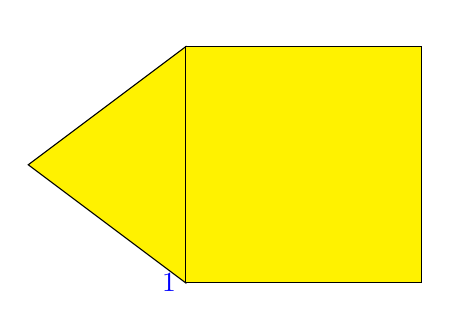
\begin{tikzpicture}
    % Mechanism to activate all labels
    \ifdefined\allLabels
        \def\vertexLabels{1}
        \def\edgeLabels{1}
        \def\faceLabels{1}
    \fi

	\def\lab{label={[blue]left:1}}
    \coordinate [label={[vertex]left:1 }](P2) at (2,-1);
    \coordinate [] (P1) at (0,0.5);
%    [label=left:\ifdefined\vertexLabels 1 \fi](P1) at (0,0.5);
    \coordinate [ label=above:\ifdefined\vertexLabels 3 \fi](P3) at (2,2);
    \coordinate [label=above:\ifdefined\vertexLabels 4 \fi](P4) at (5,2);
    \coordinate [label=below:\ifdefined\vertexLabels 5 \fi](P5) at (5,-1);

    \filldraw[face] (P1) -- (P2) -- (P3) -- cycle;
    \filldraw[face] (P2) -- (P3) -- (P4) -- (P5) -- cycle;
    \ifdefined\faceLabels
        \node at ($1/3*(P1)+1/3*(P2)+1/3*(P3)$) {I};
        \node at ($1/4*(P2)+1/4*(P3)+1/4*(P4)+1/4*(P5)$) {$\circlearrowright$};
    \fi

    \ifdefined\edgeLabels
        \drawEdge{P1}{P2}{1}
        \drawEdge{P1}{P3}{2}
        \drawEdge{P2}{P3}{3}
        \drawEdge{P3}{P4}{4}
        \drawEdge{P4}{P5}{5}
        \drawEdge{P5}{P2}{6}
    \fi

    \ifdefined\vertexLabels
        \foreach \p in {P1,P2,P3,P4,P5}{
            \fill[vertex] (\p) circle (\vSize);
        }
    \fi
\end{tikzpicture}
\end{document} 